\section{V5}
\subsection{Data Alignment}
In der Cortex-M Nomenklatur werden direkt aufeianderfolgende Bytes wie folg bezeichnet:\\

\begin{tabular}{|l|l|l|}
	\hline
	\textbf{2 Byte} & 16-Bit \textbf{Half-World} & Halbwort \\\hline
	\textbf{4 Byte} & 32-Bit \textbf{Word} & Wort \\\hline
	\textbf{8 Byte} & 64-Bit \textbf{Double-Word} & Doppelwort\\\hline 
\end{tabular}\\

Pro Operation (read oder write) k"onnen auf dem internen 32-Bit breiten Datenbuses 4 Byte gemeinsam "ubertragen werden. Sehr oft sind aber kleinere Dateneinheiten (Half-Word oder Byte) zu "ubertragen. Zudem kommt es recht h"aufig vor, dass die Daten nicht auf die 32-Bit Wortgrenze ausgerichtet sind, also als \textbf{misaligned data} im Speicher abgelegt sind. Misaligend Half-Word, Word oder Double-Word Operanden im Speicher ben"otigen somit mehr als einen \textit{Memory-Cycle}. Wenn man zum Beispiel einen Operanden von der Adresse 0x102 lesen will, wird im ersten \textit{Memory-Cycle} ein Word von der Adresse 0x100 gelesen und dann im zweiten \textit{Memory-Cycle} wird ein Word von der Adresse 0x104 gelesen. Der Operand wird dann aus den beiden gelesenen Word zusammengesetzt.

    \begin{minipage}{9cm}
    	\subsubsection{Aligned Data}
    	Operanden k"onnen mit einem \textit{Memory-Cycle} ausgelesen/geschrieben werden.
    	
    	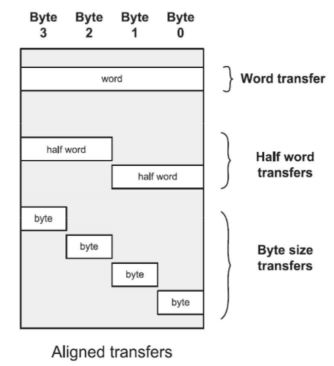
\includegraphics[width=5cm]{images/alignedData}
    \end{minipage}
    %
    \begin{minipage}{0.5cm}
    	\-\
    \end{minipage}
    %
    \begin{minipage}{9cm}
    	\subsubsection{Unaligned Data}
    	Operanden m"ussen aus mehreren \textit{Memory-Cycle} zusammengesetzt werden.
    	
    	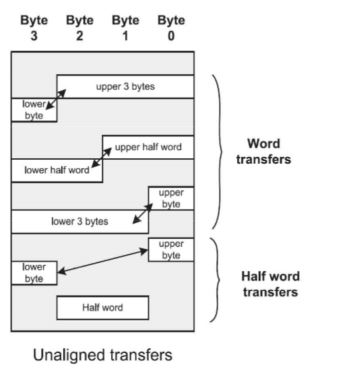
\includegraphics[width=5cm]{images/unalignedData}
    \end{minipage}
    
\subsection{Bit-Banding}
\begin{minipage}{9cm}
	\vspace{-6ex}
	Bit-Banding verwendet zwei verschiedene Regionen im Adressraum, um effektiv auf dieselben physischen Daten zu verweisen:
	\begin{itemize}
		\item Im \textit{Bit-Band Region} Speicherbereich referenziert jede Adresse genau ein einzelnes Byte an Daten, bestehend aus 8 Bits
		\item Im \textit{Bit-Band Alias} Speicherbereich wird mit jeder Adresse nur ein einzelnes Bit in der prim"aren \textit{Bit-Band Region} angesprochen.
	\end{itemize}
\end{minipage}
%
\begin{minipage}{0.5cm}
	\-\
\end{minipage}
%
\begin{minipage}{9cm}
	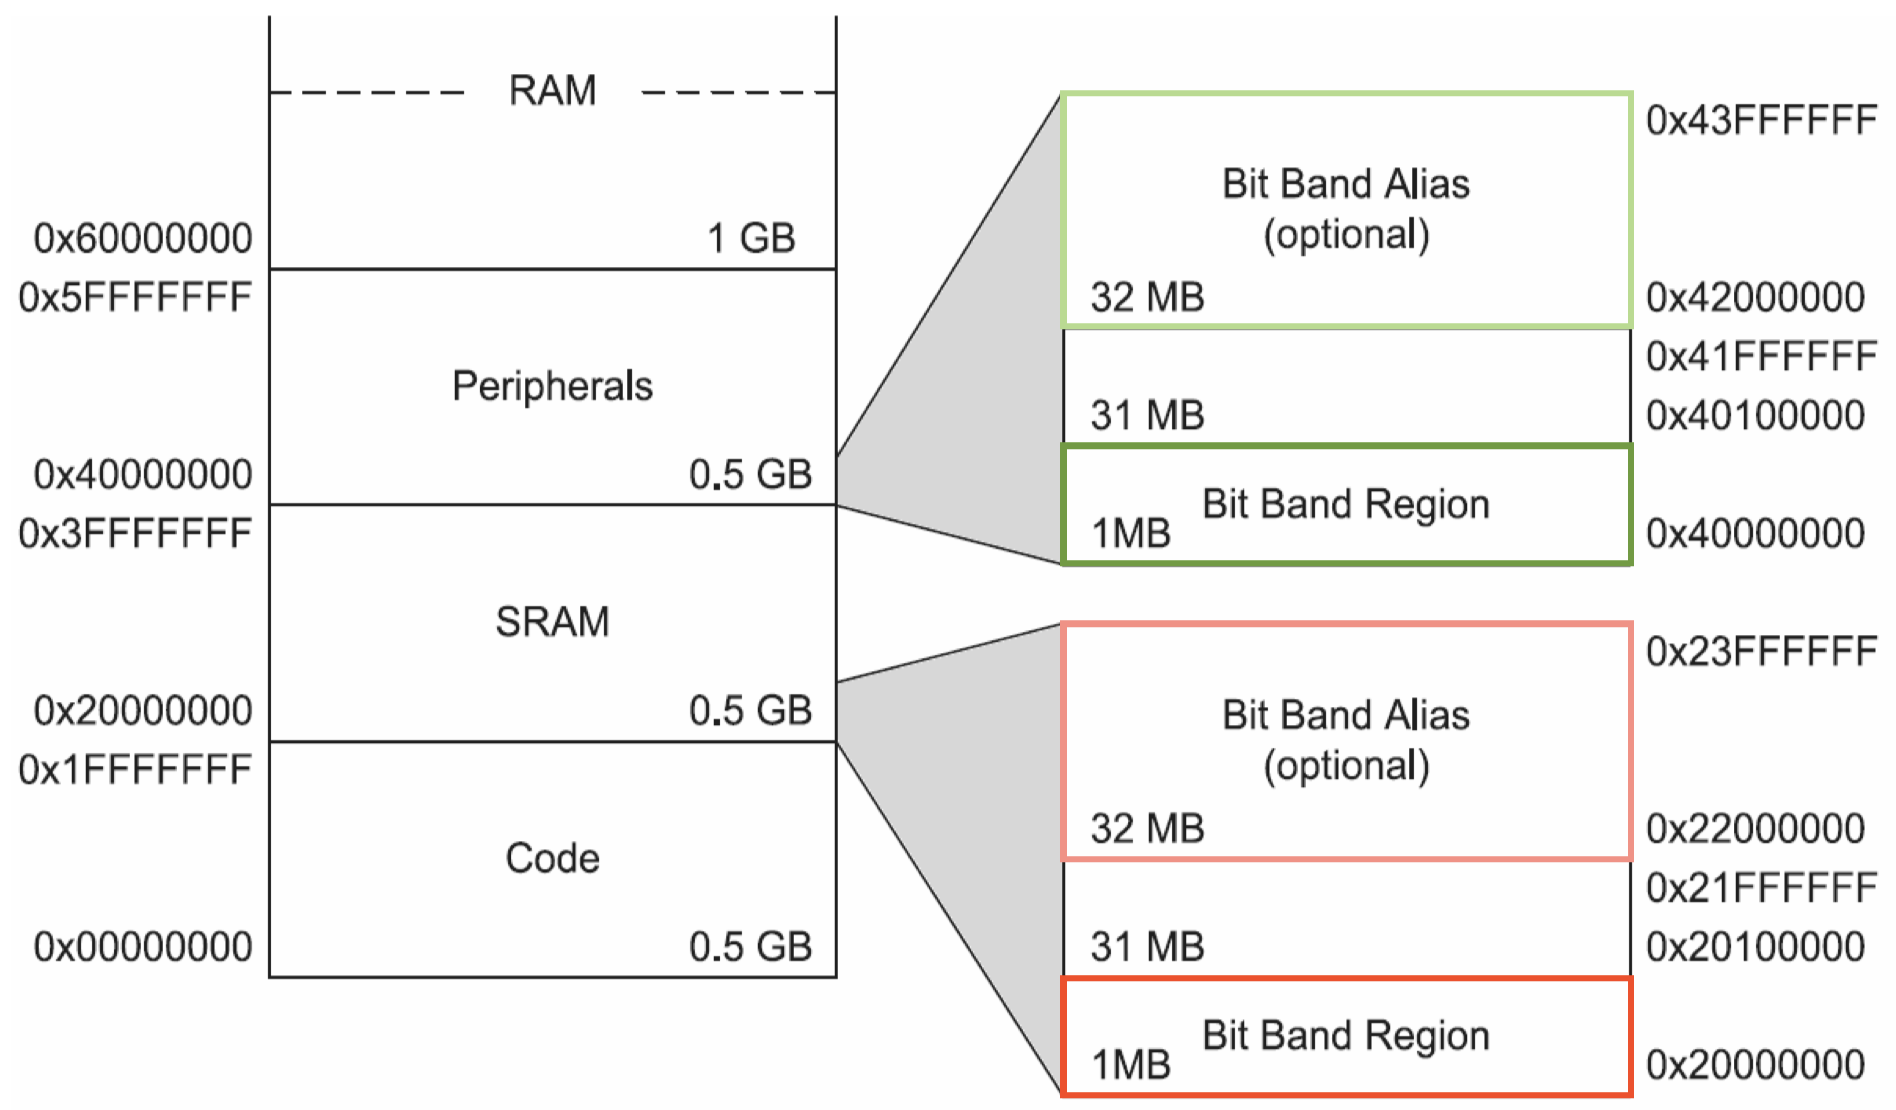
\includegraphics[width=9cm]{images/Bit-Banding}
\end{minipage}

\subsubsection{Berechnung der Adresse}
\begin{minipage}{12cm}
	\vspace{-2ex}
	\textbf{BBAA} = \textbf{BBAB} + (\textbf{MA} - \textbf{BBRB}) $\cdot 2^5$ + 4 $\cdot$ \textbf{BNr}\\
	\textbf{BNr} = [ 0x0000001F \& (\textbf{BBAA} - \textbf{BBAB}) ] $\cdot 2^{-2}$\\
	\textbf{MA} = (\textbf{BBAA} $-$ \textbf{BBAB})$\cdot 2^{-5}$ + \textbf{BBRB}\\
	
	Bei der zur"uckrechnung ist \textbf{MA} die Byte-Adresse und \textbf{BNr} immer zwischen 0-7. Wenn nun die aligned Half-Word oder aligned Word Adresse gefragt ist muss die Adresse und die Bitnummer noch dementsprechend angepasst werden.
\end{minipage}
%
\begin{minipage}{0.5cm}
	\-\
\end{minipage}
%
\begin{minipage}{6cm}
	Legende:
	\begin{tabular}{|l|l|}
		\hline
		BBAA & Bit-Band Alias Address\\\hline
		BBAB & Bit-Band Alias Base \\\hline
		MA & Memory-Address \\\hline
		BBRB & Bit-Band Region Base\\\hline
		BNr & Bit-Number\\\hline
	\end{tabular}
\end{minipage}